\chapter{Results and Discussion}\label{chapter:results}

This chapter explains the evaluation methods used for evaluating the performance of machine learning models and presents the results.

\section{Results for \textit{SSModel}}

This section presents the results for same-sentence model (\textit{SSModel}). The results are initially discussed for the model trained on training data and evaluated on development data. All experimentation such as feature selection, hyperparameter search is performed with the development data. Once the number of features to keep are fixed and the hyperparameter is exhaustively searched, the training model is used for evaluation on the test data. The results on unseen test data are considered final results. All following subsections until subsection \ref{subsec:SSFinalRes} presents the results for a model trained on training data and evaluated on development data.

%After all experimentation, an additional model is training combining training and development data. Such a model is used to evaluate the test data and the results in such a way are considered much more robust.
 
\subsection{Initial results}

\begin{figure}
\centering
\begin{minipage}{.5\textwidth}
  \centering
  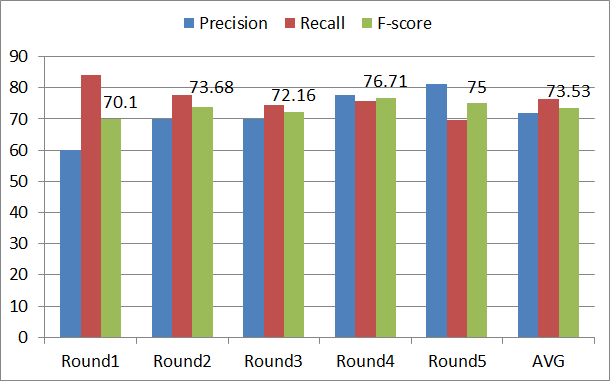
\includegraphics[width=.95\textwidth]{figures/SSInitialResultsNUniq.png}
  \caption{\textit{SSModel} non unique results}
  \label{fig:SS_NU_Initial}
\end{minipage}%
\begin{minipage}{.5\textwidth}
  \centering
  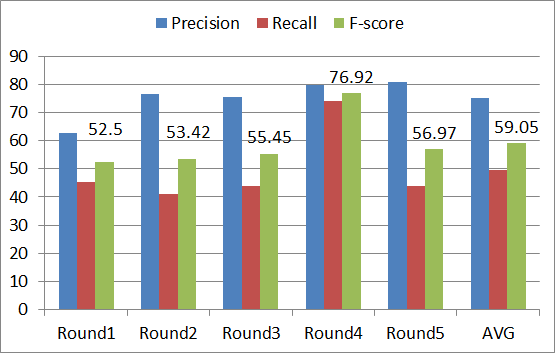
\includegraphics[width=.95\textwidth]{figures/SSInitialResultsUniq.png}
  \caption{\textit{SSModel} unique results}
  \label{fig:SS_U_Initial}
\end{minipage}
\end{figure}

As explained in Section \ref{sec:training}, 5-fold cross-validation is performed on the LocText corpus. For the details of cross-validation, refer to Section \ref{sec:training}. The primary evaluation results are shown in figures \ref{fig:SS_NU_Initial} and \ref{fig:SS_U_Initial}. Figure \ref{fig:SS_NU_Initial} shows the results of \textit{SSModel} using non unique evaluation mode (Section \ref{subsubsec:NonUniqEval}) and Fig. \ref{fig:SS_U_Initial} shows the results of \textit{SSModel} using unique evaluation mode (Section \ref{subsubsec:UniqEval}). The results are shown in terms of \textit{Precision} (\ref{subsubsec:Prec}), \textit{Recall} (\ref{subsubsec:Recal}) and \textit{F score} (\ref{subsubsec:Fscore}) for every round of cross validation and average performance is shown in the end. The \textit{F score} bars in the figures are also labeled with the actual value. The non unique average \textit{F score} for \textit{SSModel} is 73.53 and unique average \textit{F score} for \textit{SSModel} is 59.05 as shown in the figures.

\subsubsection{Experimentation}

In order to make \textit{SSModel} robust and adaptable to other corpus, a lot of experimentation was carried out. Every round of cross validation creates a model from around 30000 features on average. A lot of these features can be very specific to the LocText corpus and therefore, the efforts are made to discard unnecessary and redundant features. Following types of experiments are carried out:

\begin{itemize}

\item Leave One Out Analysis

\item Feature Weight Ranking

\item Information Gain Analysis

\end{itemize}

These experimentation results are discussed in upcoming sections. This experimentation falls into the category of feature selection broadly discussed in the section \ref{sec:featSel}.

\subsection{Results after Leave One Out Analysis}

\begin{figure}
\centering
\begin{minipage}{.5\textwidth}
  \centering
  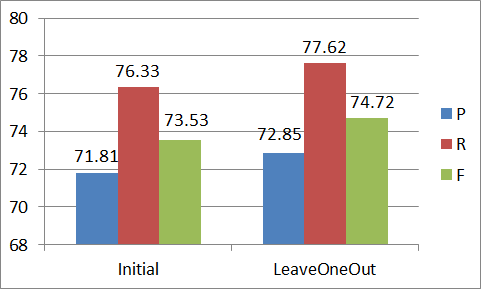
\includegraphics[width=.95\textwidth]{figures/LeaveOneOutNUniq.png}
  \caption{Non unique results comparison}
  \label{fig:LeaveOO_NU}
\end{minipage}%
\begin{minipage}{.5\textwidth}
  \centering
  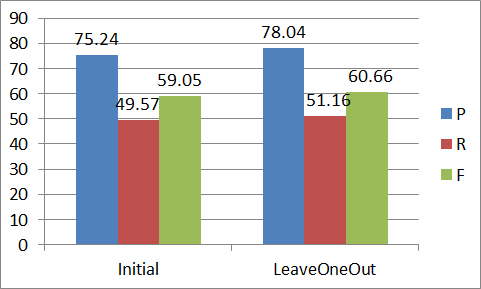
\includegraphics[width=.95\textwidth]{figures/LeaveOneOutUniq.png}
  \caption{Unique results comparison}
  \label{fig:LeaveOO_U}
\end{minipage}
\end{figure}

The theoretical aspects of Leave One Out approach are discussed in detail in Subsection \ref{subsec:LeaveOneOut}. To summarize this approach, the feature generators or functions that generates the features are greedily discarded to improve the performance of the model.

Figure \ref{fig:LeaveOO_NU} and \ref{fig:LeaveOO_U} show the comparison between the results of initial model and after performing the LeaveOneOut experimentation.  The \textit{Precision}, \textit{Recall} and \textit{F score} are denoted by P, R and F respectively. Figure \ref{fig:LeaveOO_NU} shows the comparison using non-unique evaluation mode and \ref{fig:LeaveOO_U} shows the comparison using unique evaluation mode. As shown in the figures, the average \textit{F score} increased from 73.53 to 74.72 for non-unique evaluation and from 59.05 to 60.66 for unique evaluation. In addition to the increase in the performance, there has been some reduction in the average number of features. The initial model used around 30900 features on average in every round of the cross validation whereas the model refined after LeaveOneOut experimentation uses 29000 features on average in every round, therefore reducing the number of features by 1900 for every round of the cross-validation.

\subsection{Results after Feature Weight Ranking}

The Feature Weight Ranking (FWR) approach, discussed in detail in Subsection \ref{subsec:FWR}, uses the weights of the features for feature selection. The support vector machine (SVM), while creating a hyperplane to separate positive and negative instances in the training data, learns the weights for the features. These weights can be extracted from the learned model using a perl script \cite{svmlightonline}. 


\begin{figure}
\centering
\begin{minipage}{.5\textwidth}
  \centering
  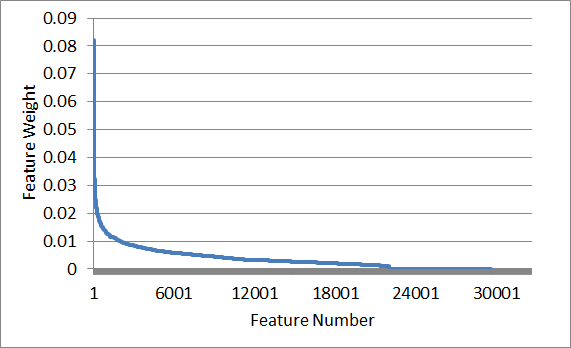
\includegraphics[width=.95\textwidth]{figures/FWRWeightDist.png}
  \caption{Feature weight distribution}
  \label{fig:FWRWeightDist}
\end{minipage}%
\begin{minipage}{.5\textwidth}
  \centering
  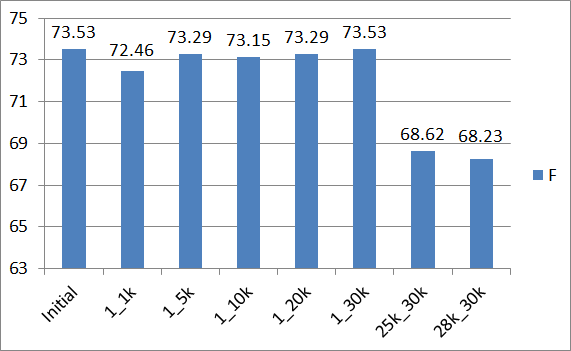
\includegraphics[width=.95\textwidth]{figures/FWRPerformance.png}
  \caption{FWR Performance comparison}
  \label{fig:FWRPerfComp}
\end{minipage}
\end{figure} 

For each round of cross-validation, a model is learned and therefore, the feature weights can be extracted for every round. Figure \ref{fig:FWRWeightDist} shows the distribution of weights for features of round 1, from highest weighted feature to lowest weighted feature. The weights of the features in other folds follow similar distribution. As shown in figure, there are very less features with higher weights and most of the features have comparatively lower weights.

Figure \ref{fig:FWRPerfComp} shows the comparison of performance of various FWR (Feature Weight Ranking) models with initial model. Only average \textit{F scores} are shown for comparison. The model \textit{1\_1k} implies that the model is trained using 1000 highest weighted features from every round of cross validation. Similar terminology applies for rest of the FWR models shown in the figure. None of the FWR models have a higher performance than the initial model. The performance of FWR model with first 1000 features (\textit{1\_1k}) is lower than FWR model with first 5000 features (\textit{1\_5k}). It is also seen that the performance drops for first 10000 (1\_10k) features and then again increases for 20000 (1\_20k) and 30000 (1\_30k) features. This trend invalidates the intuition that higher weighted features should result in higher performance and addition of lower weighted features should decrease the performance. In our case, addition of features ranked 10000 to 20000 have actually increased the performance. The FWR model consisting of lowest 2000 features in every round (\textit{28k\_30k}) also has considerable performance and cannot be discarded as useless. Owing to all these problems, this approach was not experimented further.
 
\subsection{Results after Information Gain Analysis}\label{subsec:SS_IG}

Information gain is widely used technique for the purpose of feature selection. The theoretical background for calculating information gain can be found in Subsection \ref{subsec:IG}. The information gain is calculated for features in every round of cross validation and analysis is done similar to the analysis based on feature weights.

\begin{figure}
\centering
\begin{minipage}{.5\textwidth}
  \centering
  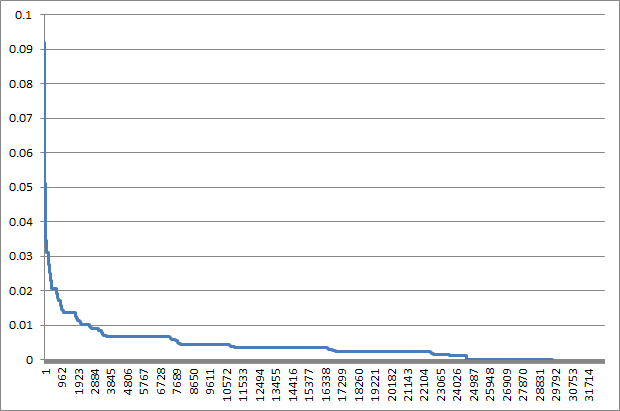
\includegraphics[width=.95\textwidth]{figures/IGDistr1.png}
  \caption{Information Gain distribution}
  \label{fig:IGDist}
\end{minipage}%
\begin{minipage}{.5\textwidth}
  \centering
  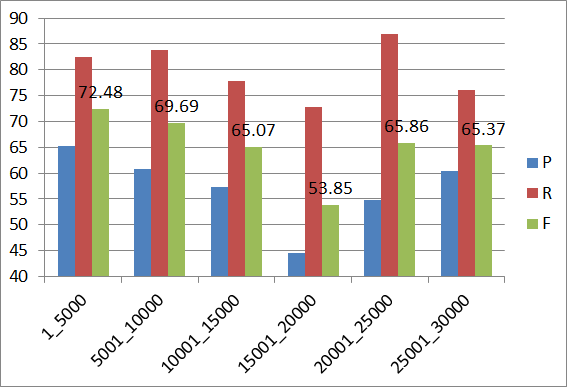
\includegraphics[width=.95\textwidth]{figures/IG5kSlabsComp.png}
  \caption{IG models with 5k slabs}
  \label{fig:IG5kComp}
\end{minipage}
\end{figure} 

Figure \ref{fig:IGDist} shows the information gain of the features used in round 1. The distribution of information gain is similar to the distribution of feature weights with minor difference that the feature weight distribution is much smoother than the distribution of information gain. To analyze the effectiveness of features with different information gain, an experiment was conducted by dividing the features into slabs of 5000 features depending on their information gain. Figure \ref{fig:IG5kComp} shows the average performance of various models trained with slabs of 5000 features. The model \textit{1\_5000} uses the first 5000 features with best information gain, the model \textit{5001\_10000} uses next 5000 features and so on. As seen in the figure, none of the 5k models have exceptionally low performance except model \textit{15001\_20000}. This further consolidates the finding of Joachims et al. \cite{joachims1998text} that all features have some or other information and aggressive feature selection might not result in manifold increase in the performance.

Further experiments were carried out using some of the features with best information gain. For this purpose, first 5000 features were considered. Different models were trained using first 1000, 2000, 4000 and 5000 features and their performance was compared with the initial model.  Figure \ref{fig:IG_5k_NU} shows the comparison of models using non unique evaluation mode and \ref{fig:IG_5k_U} shows the comparison of models using unique evaluation mode. As seen in Fig. \ref{fig:IG_5k_U}, the model with first 2000 features registers much better performance than the initial model. For the same model, the non unique comparison in Fig. \ref{fig:IG_5k_NU} shows highest increase in the \textit{Recall} from 73.83 to 84.74.

\begin{figure}
\centering
\begin{minipage}{.5\textwidth}
  \centering
  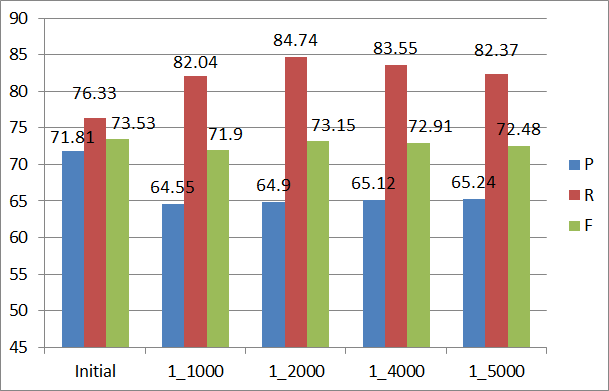
\includegraphics[width=.95\textwidth]{figures/IGFirst5k_NU.png}
  \caption{IG non unique comparison}
  \label{fig:IG_5k_NU}
\end{minipage}%
\begin{minipage}{.5\textwidth}
  \centering
  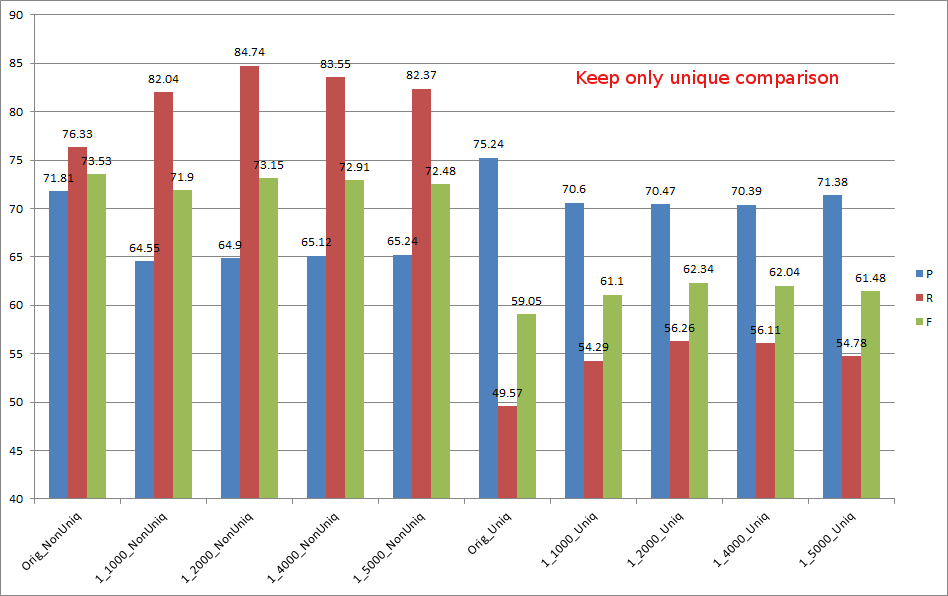
\includegraphics[width=.95\textwidth]{figures/IGFirst5k_U.png}
  \caption{IG unique comparison}
  \label{fig:IG_5k_U}
\end{minipage}
\end{figure} 


As described previously, the features are generated by feature generators or functions. Note that the term feature generator and feature functions mean the same and used interchangeably in the explanation ahead. In order to discard bad features, the solution is to discard the feature generators that decrease performance. A feature generator can generate a lot of features and the options is to either keep all of them or discard all of them. Hence, it was necessary to trace back the feature generators from the features. Once the feature generators are located, other features generators can be discarded and the performance of such a model can be observed.

To trace back the feature generators, every feature was given a label indicating the feature generator that produced it. There were a total of 109 feature generators and to choose some of them, it was necessary to assign a statistic to each feature generator. Following criteria were used for selection of feature generators:

\begin{itemize}

\item \textbf{Total information gain:} For every feature generator, the information gain of its features in all 5 rounds of cross validation was summed up to produce a number called total information gain.

\item \textbf{Number of features:} The number of features produced by each feature generator.

\item \textbf{Average information gain:} Average information gain for a feature generator was calculated by dividing the total information gain by number of features produced by it.

\item \textbf{Minimum information gain:} Minimum information gain for a feature generator is equal to minimum of information gains of its features.

\item \textbf{Maximum information gain:} Maximum information gain for a feature generator is equal to maximum of information gains of its features.

\end{itemize}

Using these 5 statistics, an exhaustive search was conducted to select the best model. For every statistic, a model was trained and evaluated using some or all of the feature generators. For example, if the statistic total information gain is considered, 109 models were trained and evaluated. The models were named as TIG\_1 to TIG\_109. TIG\_1 implies that the criteria total information gain (TIG) is used to choose a single feature generator with best total information gain. Similarly, TIG\_10 indicates a model trained using 10 feature generators with highest total information gain. Such experiments were conducted for all of the 5 criteria/statistics mentioned above. Some of the interesting results are explained in figures \ref{fig:AvgIG} and \ref{fig:MinIG}.

\begin{figure}
\centering
\begin{minipage}{.5\textwidth}
  \centering
  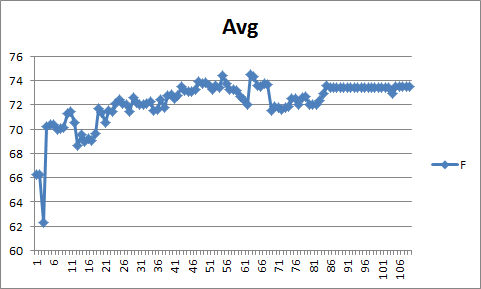
\includegraphics[width=.95\textwidth]{figures/AvgIGAnalysis.png}
  \caption{Average IG experiments}
  \label{fig:AvgIG}
\end{minipage}%
\begin{minipage}{.5\textwidth}
  \centering
  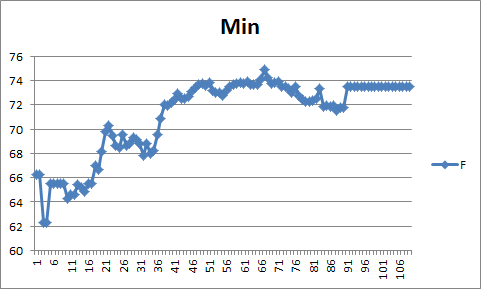
\includegraphics[width=.95\textwidth]{figures/MinIGAnalysis.png}
  \caption{Minimum IG experiments}
  \label{fig:MinIG}
\end{minipage}
\end{figure} 

Figures \ref{fig:AvgIG} and \ref{fig:MinIG} shows the variation of \textit{F scores} of different models created using average information gain and minimum information gain respectively. For average information gain, the models are addressed as Avg\_1 to Avg\_109 depending on the number of feature generators used for training. Similarly, for minimum information gain, the models are addressed as Min\_1 to Min\_109 depending on the number of feature generators used for training. The last point in the line graph Avg\_109 or Min\_109 shows the performance of model using all 109 feature generator, i.e., without any feature selection. The performance of Avg\_109 and Min\_109, therefore, is equal to the performance of initial model which is a \textit{F score} of 73.53 according to non unique evaluation method. In Fig. \ref{fig:AvgIG}, there are 3 models, viz., Avg\_55, Avg\_63 and Avg\_64 that have better performance than the initial model (Avg\_109). Similarly, in the figure \ref{fig:MinIG}, there are 3 models, viz., Min\_66, Min\_67 and Min\_68 that have better performance than the initial model (Min\_109). These 6 models were selected and analyzed.

\begin{figure}
\centering
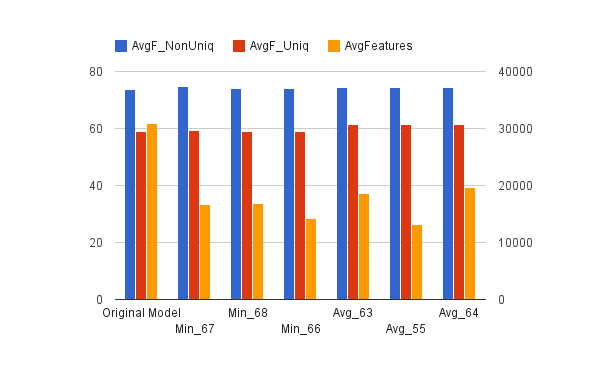
\includegraphics[scale=0.6]{figures/6ModelsComparison.png}
\caption{Comparison of selected models with initial model}\label{fig:6ModelsComp}
\end{figure}

As shown in Fig. \ref{fig:6ModelsComp}, Avg\_55 has near to best performance with respect to non unique evaluation mode, best performance with respect to unique evaluation mode and highest reduction in the number of features. The average number of feature for Avg\_55 is around 13230 compared to 30900 in the initial model. Therefore, Avg\_55 models was selected as the best \textit{SSModel}.


\subsection{Hyperparameter search results}

Exhaustive hyperparameter search was conducted for the selected model Avg\_55. The hyperparameter for support vector machine model is the regularization parameter $\mathbf{C}$ which determines the trade-off between training error and test error as explained in Subsection \ref{subsec:RegPar}. Experiments were conducted for finding the best regularization parameter by varying $\mathbf{C}$ from 0.0000 to 2.0000 with the steps of 0.0005. A value of 0.0005 was found to be the best hyperparameter value which results in increase in performance of 1.76 with respect to unique evaluation mode. The hyperparameter search was done to  maximize the performance with respect to unique evaluation mode.

\begin{figure}
\centering
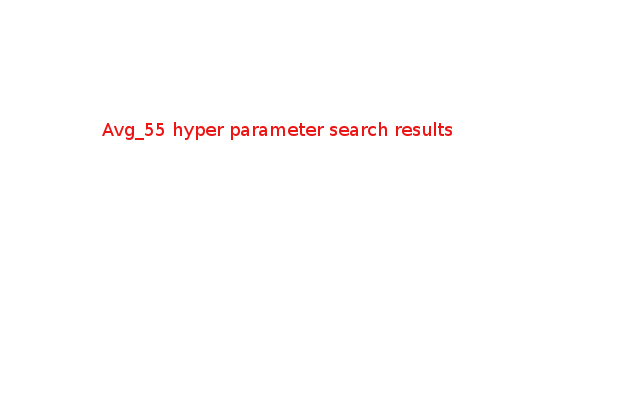
\includegraphics[scale=0.6]{figures/SSModelRegPar.png}
\caption{Results before and after hyperparameter search}\label{fig:SSModelRegPar}
\end{figure}

\subsection{Final Results}\label{subsec:SSFinalRes}

\begin{figure}
\centering
\begin{minipage}{.5\textwidth}
  \centering
  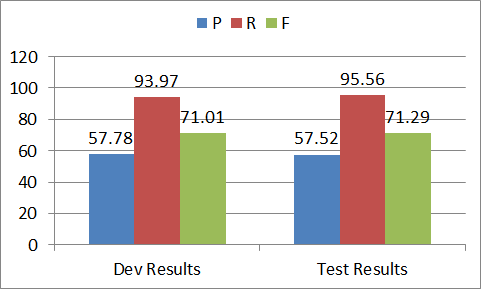
\includegraphics[width=.95\textwidth]{figures/CompDevTestResultsNonUniq.png}
  \caption{Non unique mode results}
  \label{fig:SS_DevTest_NU}
\end{minipage}%
\begin{minipage}{.5\textwidth}
  \centering
  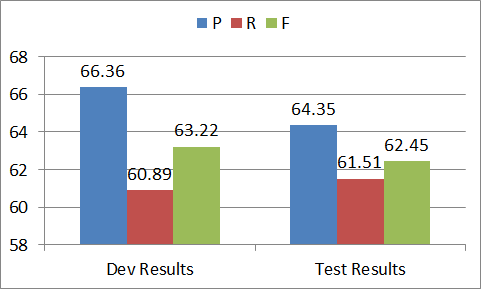
\includegraphics[width=.95\textwidth]{figures/CompDevTestResultsUniq.png}
  \caption{Unique mode results}
  \label{fig:SS_DevTest_U}
\end{minipage}
\end{figure}

The optimal \textit{SSModel} trained after feature selection and hyperparameter search is finally evaluated on unseen test data. Since the test data is not touched during tuning of the model, the evaluation on test data is considered a robust estimate of the model performance and hence, can be termed as final results for \textit{SSModel}.

Figure \ref{fig:SS_DevTest_NU} shows the comparison between average results of the optimal \textit{SSModel} on development set termed as "Dev Results" and test set termed as "Test Results". The results in Fig. \ref{fig:SS_DevTest_NU} are computed using non unique mode of evaluation. As shown in figure, the evaluation performance on the test set is nearly equal to the evaluation performance on the development set. While the average \textit{F score} for evaluation on development set is 71.01, the average \textit{F score} for evaluation on the test set is 71.29.

Figure \ref{fig:SS_DevTest_U} shows similar comparison between evaluation performance on the development set and the test set, but using unique mode of evaluation. Similar to the trends in Fig. \ref{fig:SS_DevTest_NU}, the evaluation performance on the test set is nearly equal to the evaluation performance on development set. As shown in the figure, the average \textit{F score} for evaluation on development set is 63.22 whereas the average \textit{F score} for evaluation on the test set is 62.45.

\section{Results for \textit{DSModel}}

This section discusses the evaluation of performance of the different-sentence model (\textit{DSModel}). The goal of the \textit{DSModel} is to extract the protein-location relations in which either of the entity is present in a different sentence. The overall objective of using two different models, viz. \textit{SSModel} and \textit{DSModel} is to extract as many protein-location relations as possible. 

The evaluation of performance of the \textit{DSModel} is, in a way, dependent on the predictions of the \textit{SSModel}. If unique mode of evaluation (Section \ref{subsubsec:UniqEval}) is considered, then it may happen that a particular relation predicted by the \textit{DSModel} is already predicted by the \textit{SSModel}. In this particular case, the \textit{DSModel} is not adding any extra information to the set of predictions. Therefore, utmost care is taken while evaluating the results of the \textit{DSModel}. Several evaluation criteria are developed to understand how the \textit{DSModel} is supplementing the set of predictions. These evaluation criteria are:

\begin{itemize}

\item \textit{SVM Performance:} This criteria describes the performance of the SVM model. This is exactly the same as non unique mode of the evaluation (Subsection \ref{subsubsec:NonUniqEval}).

\item \textit{Unique performance:} This criteria compares the set of predictions of the \textit{DSModel} with the unique set of relations for the document in the corpus. This is exactly same as unique mode of the evaluation (Subsection \ref{subsubsec:UniqEval}).

\item \textit{Manipulated prediction:} In this evaluation mode, the predictions of the \textit{DSModel} are manipulated to some extent. The intuition behind this manipulation is, if a relation is predicted positive by the \textit{SSModel} (in other words, the \textit{SSModel} predicts that the entities in the relation are related and present in the same sentence), then it is highly unlikely that the same entities could be related in a different-sentence relation. Therefore, if a relation predicted by the \textit{DSModel} is found in the list of positive predictions by \textit{SSModel}, then that particular relation prediction is manipulated into a negative prediction, irrespective of whether it was a positive prediction or a negative prediction earlier. 

\item \textit{Combined evaluation:} The predictions of \textit{SSModel} and \textit{DSModel} are combined in a unique list of predictions. It also means that if a relation is predicted both by \textit{SSModel} and \textit{DSModel}, then the prediction is added to the unique list only once. This unique list of predictions is then compared with the unique list of relations for every document in the corpus and the results are computed. 

\end{itemize}

\subsection{Initial Results}

\begin{figure}
\centering
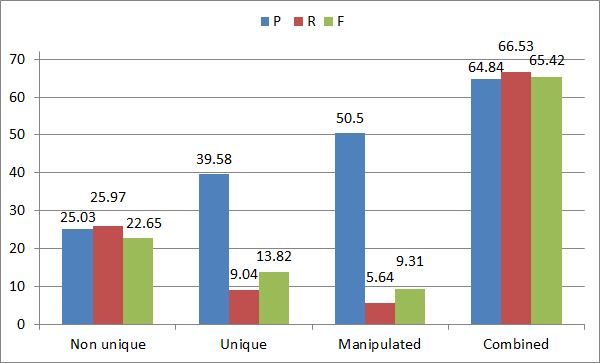
\includegraphics[scale=0.7]{figures/DSInitialResults.png}
\caption{Initial results of \textit{DSModel}}\label{fig:DSInitial}
\end{figure}

Figure \ref{fig:DSInitial} shows the initial results of the \textit{DSModel}. These are the results prior to any experimentation for feature selection or hyperparameter search. The results are shown in the figure according to various evaluation criteria explained in the previous section. For combined evaluation, the predictions of the \textit{DSModel} are combined with predictions of best performing \textit{SSModel}, i.e., the predictions generated by Avg\_55 model trained using optimal hyperparameter.

\subsection{Need for optimizing combined evaluation}

During various experimentation, it was found out that the non unique performance does not correlate well with combined evaluation performance. In other words, if the efforts are made to maximize non-unique or unique performance of the \textit{DSModel}, then it does not necessarily optimizes the combined performance.  This may happen due to the reason that the model with optimal non-unique performance produces more repeated predictions that are already predicted by the \textit{SSModel}. Therefore, it was decided for further experimentation that efforts would be made to optimize the combined performance rather than unique or non-unique performance.

The experimentation performed on the \textit{DSModel} was similar to the experimentation performed on the \textit{SSModel}. Three experiments, viz. Leave One Out Analysis, Feature Weight Ranking and Information Gain Analysis, were carried out for feature selection. Following subsections describe the results of these experiments:

\subsection{Results after Leave One Out Analysis}

The theoretical background for Leave One Out approach is discussed in Subsection \ref{subsec:LeaveOneOut}. In this approach, the feature generators or functions are greedily discarded to produce the best possible performance.

\begin{figure}
\centering
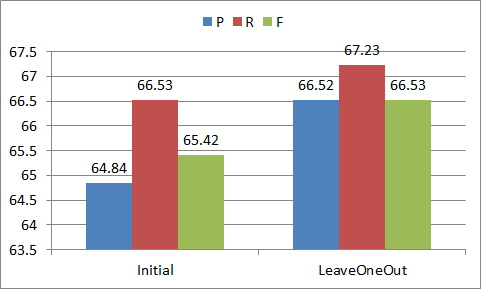
\includegraphics[scale=0.8]{figures/DSLeaveOneOutComb.png}
\caption{Effect of Leave One Out Analysis on \textit{DSModel}}\label{fig:DSLeaveOO}
\end{figure}

Figure \ref{fig:DSLeaveOO} shows the effect of Leave One Out experimentation. The \textit{F score} for combined evaluation increased from 65.42 to 66.53. The total number of features used by initial model for 5 rounds of cross-validation was 310512 (62000 features per round of cross-validation on average). After Leave One Out experimentation, the total number of features for 5 rounds dropped to 201475 (average 40295 features per round), thereby reducing the number of features to a good extent.

\subsection{Results after Feature Weight Ranking}

The Feature Weight Ranking (FWR) approach is discussed in detail in Subsection \ref{subsec:FWR}. This approach uses the feature weights learned by Support Vector Machine (SVM), for the purpose of feature selection.

\begin{figure}
\centering
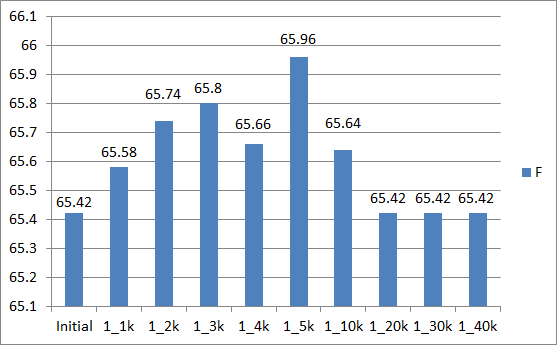
\includegraphics[scale=0.7]{figures/DSFWRResults.png}
\caption{Effect of Feature Weight Ranking approach on \textit{DSModel}}\label{fig:DSFWR}
\end{figure}

Figure \ref{fig:DSFWR} shows the comparison between average \textit{F score} for combined evaluation mode. Initial model shows the performance before any experimentation. The model 1\_1k implies that 1000 highest weighted features from every round of cross validation are used for training the model. Similarly, the model 1\_20k implies that 20000 highest weighted features from every round of cross validation are used for training the model. As shown in Fig. \ref{fig:DSFWR}, the model 1\_5k register the best performance. However, the performance obtained is lower than the best performance obtained by LeaveOneOut experimentation and therefore, this approach was not further investigated. The weights of the features followed similar distribution as followed by the weights of the features for \textit{SSModel} in Fig. \ref{fig:FWRWeightDist}.

\subsection{Results after Information Gain Analysis}


Information gain analysis is most widely used approach for the purpose of feature selection. The theoretical aspects of Information Gain Analysis are discussed in Subsection \ref{subsec:IG}. The approach is also widely discussed for SSModel in Subsection \ref{subsec:SS_IG}. 

\begin{figure}
\centering
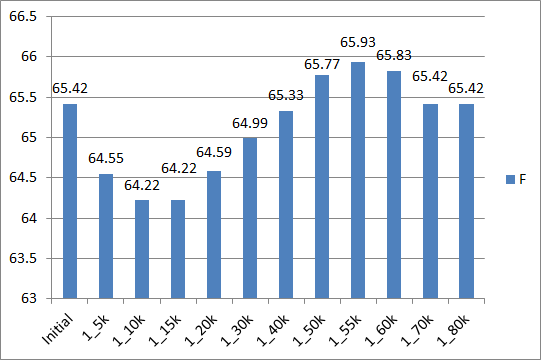
\includegraphics[scale=0.7]{figures/DSIGResults.png}
\caption{Effect of Information Gain Analysis on \textit{DSModel}}\label{fig:DSIG}
\end{figure}


The initial model has close to 62000 average features for every round of cross validation. Information gain is calculated for every feature. The information gain for the features in every round follows similar distribution as observed in Fig. \ref{fig:IGDist}. 

Figure \ref{fig:DSIG} shows the comparison between different models using information gain analysis. The initial model represents the model before information gain analysis experiments. The model 1\_5k implies that 5000 features with best information gain are selected for every round of cross validation and the model is trained. As seen in the figure, the performance of the IG (information gain) models continue to rise from 1\_5k to 1\_55k. The model trained using best 55000 features (1\_55k) produces the best performance and surpasses the performance of the initial model. Since there are around 60000 features per round of cross validation and 55000 features are required for best performing model implies the fact that the features with low information gain are equally important for \textit{DSModel}. Since this approach played an important role in improving the performance of \textit{SSModel} in addition to reducing the number of features, it was decided to investigate this approach further.

As discussed in Section \ref{subsec:SS_IG}, the features have to be traced back to the feature generators that produce them. These feature generators can then be discarded in order to improve the performance and reduce the number of features. As in the case of the \textit{SSModel}, the feature generators were assigned a statistic and experiments were carried out using these statistics. Following statistics were used for every feature generator:

\begin{itemize}

\item \textit{Total information gain}

\item \textit{Number of features}

\item \textit{Average information gain}

\item \textit{Minimum information gain}

\item \textit{Maximum information gain}

\end{itemize}


These 5 statistics were used for conducting an exhaustive search. For every statistic, a model was trained and evaluated using some or all of the feature generators. For the \textit{DSModel}, there are 132 feature generators, i.e., 132 functions generate the features used for training the \textit{DSModel}. In every experiment, these 132 feature generators were sorted according to some statistic and some of them were selected for training the model. For example, in the case of using average information gain as a feature generator statistic, the feature generators were arranged from highest average information gain to lowest average information gain. If only 10 of these feature generators are used for training the model, such a model is called Avg\_10. Similarly, if 50 of the best feature generators are used for training the model, the model is called Avg\_50. The models from Avg\_1 to Avg\_132 were tested for average information gain analysis. Similarly, for minimum information gain analysis, the models from Min\_1 to Min\_132 were tested.

\begin{figure}
\centering
\begin{minipage}{.5\textwidth}
  \centering
  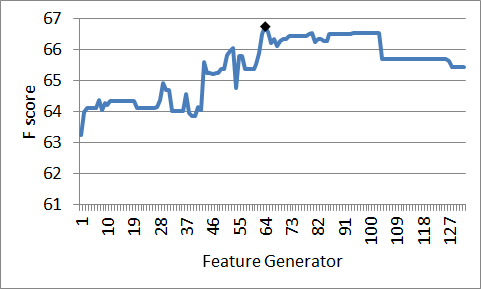
\includegraphics[width=.95\textwidth]{figures/DSAvgAnalysis.png}
  \caption{Average analysis results}
  \label{fig:DS_AvgAnalysis}
\end{minipage}%
\begin{minipage}{.5\textwidth}
  \centering
  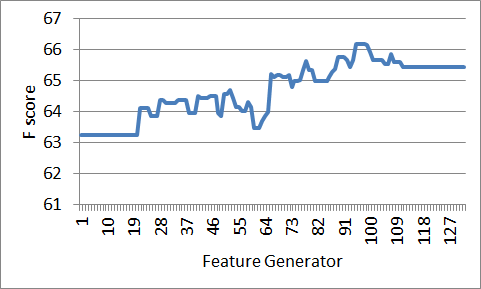
\includegraphics[width=.95\textwidth]{figures/DSMinAnalysis.png}
  \caption{Min IG analysis results}
  \label{fig:DS_MinAnalysis}
\end{minipage}
\end{figure}

Figure \ref{fig:DS_AvgAnalysis} shows the results of average information gain analysis and \ref{fig:DS_MinAnalysis} shows the results of minimum information gain analysis. As seen in Fig. \ref{fig:DS_AvgAnalysis}, the Avg\_64 model registers the best performance with a \textit{F score} of 66.73. This model also reduces the number of features from 310512 to 92514 for 5 rounds of cross validation (reduction of average number of features per round from 62000 to 18500). Since this model registers the best performance and massively reduces the number of features, this model was considered as the best model from feature selection experiments.

\subsection{Hyperparameter search results}

The optimal model Avg\_64 was tested for optimal hyperparameter. Exhaustive hyperparameter search was carried out with hyperparameter ranging from 0.0000 to 2.0000 with the steps of 0.0005. Before the exhaustive searching, the hyperparameter used was 0.0065. After the exhaustive search, the same hyperparameter registered the best performance. Therefore, no change was made for the value of hyperparameter.

\subsection{Final Results}

After rigorous feature selection and hyperparameter search, the optimal \textit{DSModel} was used for evaluation of unseen test data.

\begin{figure}
\centering
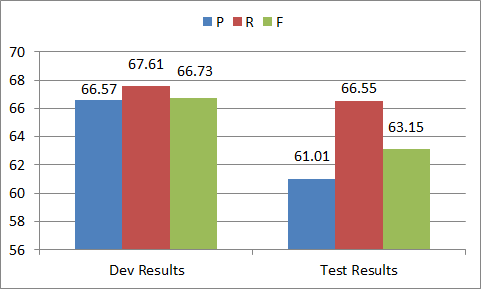
\includegraphics[scale=0.7]{figures/DSFinalResults.png}
\caption{Final evaluation on test set}\label{fig:DSFinal}
\end{figure}

Figure \ref{fig:DSFinal} shows the comparison between results on development set and test set. The \textit{F score} on development set is 66.73 while that on test set is 63.15.

%\section{Results for CombinedModel}

\section{Assessment of Performance evaluation results}

%  Explain about statistical significance tests